%
% Copyright(c) 2016 Taikai Takeda <297.1951@gmail.com> All rights reserved.
%
\section{HMM}
HMM (Hidden Markov Model) has been widely used for from gene alignment to speech recognitions. Let us introduce simple HMM before presenting Pairwise HMM.

\subsection{Formulation}
Let $\mathcal{D}=\vec{X} = (X_1, ..., X_T)$ and $\vec{Z} = (Z_1, ..., Z_T)$ be, respectively, observed and hidden random variables. 

The graphical model of HMM is shown in Fig.\ref{fig:hmm_graph}. We will present formal definitions here.
Let $\mathcal{A}$ be a set of simbols and a set of hidden states be $\mathcal{S}$.
Input data is a set of sequences, $\vec{x} = (\vec{x}^1, ..., \vec{x}^{N})$ where $n$-th sequence $\vec{x}^n \in \mathcal{A}^{T_n}$ is $T_n$ is the length of the sequence.
Similarly, hidden states are denoted as $\vec{z} = (\vec{z}^1, ..., \vec{z}^{N})$ where $n$-th sequence $\vec{z}^n \in \mathcal{S}^{T_n}$. Note that we sometimes omit superscript $n$ when concentrating on a single sequence for the sake of notational simplicity.
The corresponding joint disribution has the form
\begin{eqnarray}
  p(\vec{X}, \vec{Z} | \vec{\theta}) = p(Z_1 | \vec{\alpha}) \prod_{t=2}^T p(Z_t|Z_{t-1}, \vec{\beta}) \prod_{t=1}^T p(X_t | Z_t, \mathbf{\phi})
\end{eqnarray}
where $\mathbf{\theta} = \{\mathbf{\alpha}, \mathbf{\beta}, \mathbf{\phi} \}$. $p(Z_1| \vec{\alpha})$ , $p(Z_t|Z_{t-1}, \mathbf{\beta})$ and $p(X_t|Z_t, \mathbf{\phi})$ are an initial probability, a transition probability, an emission probability, respectively.
They are described, respectively, as $p(Z_1 = k, \vec{\alpha}) = \alpha_k$, $p(Z_t = k|Z_{t-1}=j, \mathbf{\beta}) = \beta_{jk}$ and $p(X_t|Z_t = k, \mathbf{\phi}) = p(X_t|\phi_k) = \psi_{tk}$ \footnote{MEMO: define it later (not in this subsection)}. 
$\vec{\alpha} = \{\alpha\}_k$ is $K-$dimensional vector and $\mathbf{\beta} = \{\beta\}_{jk}$ is $K \times K$ matrix where $K$ is the number of hidden states

\begin{figure}
  \centering
  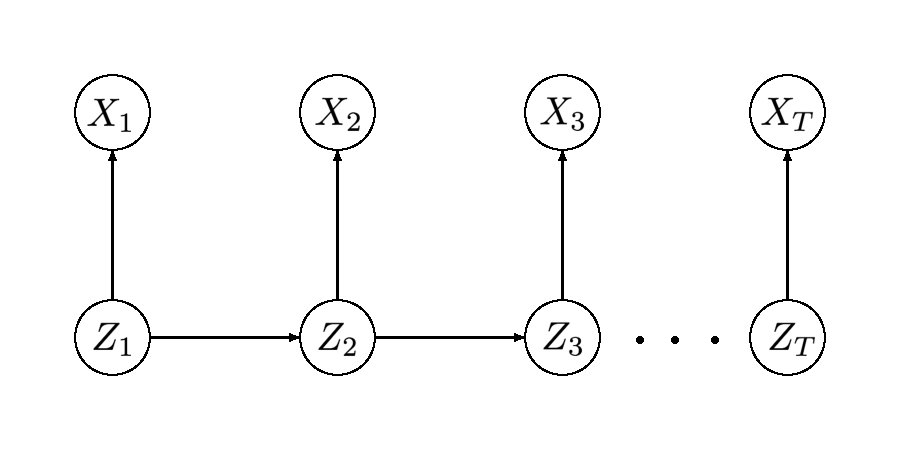
\includegraphics[width=.8\linewidth]{hmm_graph.pdf}
  \caption{{\bf Grahpical Model of HMM}}
  \label{fig:hmm_graph}
\end{figure}

\subsection{Forward-Backward Algorithm}
We here discuss how to compute the smoothed marginal $p(z_t = j| \vec{x})$ and tghe smoothed two-sliced marginal $p(z_{t-1},z_t| \vec{x})$.\footnote{Note that in online setting, we can only compute $p(z_t = j| \vec{x_{1:t}})$, so called filtered marginal, but we concentrate on the offline setting here.}

Taking a look at the graphical model in Fig(), we can see conditioning on $z_t$ eable to decompose joint distribution into two parts: the past and the future. 
\begin{eqnarray}
p(z_t= k| \mathbf{x}) \propto p(z_t=k, \mathbf{x}_{t+1:T}| \mathbf{x}_{1:t})  \propto p(z_t=k|\mathbf{x}_{1:t}) p(\mathbf{x}_{t+1:T}|z_t=k)
\end{eqnarray}
Let us define forward variables $f_{t,k} = p(z_t = k | \vec{x}_{1:t})$, the bilief of the state given all the previous sequence. 
Also, define backward variables $b_{t,k} = p(\mathbf{x}_{t+1:T}|z_t=k)$, the conditional likelihood of future evidence give the hidden staetes $z_t$.
Forward variables are efficiently computed using dynamic programming. The base case and the recursive relationship is given as follows:
\begin{eqnarray}
  f_{t,k} &=& p(z_t = k | \vec{x}_{1:t}) \nonumber \\
          &=& \frac{p(z_t = k, x_t|\vec{x}_{1:t-1})}  {p(x_t|\vec{x}_{1:t-1})} \nonumber \\  
          &=& \frac{p(x_t|z_t=k, \cancel{\vec{x}_{1:t-1}})p(z_t = k|\vec{x}_{1:t-1})}  {p(x_t|\vec{x}_{1:t-1})} \nonumber \\  
          &=& \frac{p(x_t|z_t=k) \sum_{j=1}^K p(z_t = k | z_{t-1} = j)p(z_{t-1} = j|\vec{x}_{1:t-1})}  {p(x_t|\vec{x}_{1:t-1})} \nonumber \\  
          &=& p(x_t| z_t = k) \sum_{j=1}^K  \beta_{j,k} f_{t-1,k} \\
  f_{1, k} &=& p(z_1 = k) = \alpha_k
\end{eqnarray}
\footnote{MEMO: should we define emission notation e.g. $\psi_{t,k}$}
Similarly, backward variables are computed using following equations:
\begin{eqnarray}
b_{t-1,j} &=& p(\vec{x}_{t:T}|z_{t-1}=j) \nonumber \\
          &=& \sum_{j=1}^K p(\vec{x}_{t:T}, z_{t}=j| z_{t-1}=j) \nonumber \\
          &=& \sum_{j=1}^K p(z_{t}=k| z_{t-1}=j) p(\vec{x}_{t:T}| z_t=k, \cancel{z_{t-1}=j}) \nonumber \\
          &=& \sum_{j=1}^K p(z_{t}=k| z_{t-1}=j) p(x_t|z_t=k) p(\vec{x}_{t+1:T}| z_t=k) \nonumber \\
          &=& \sum_{j=1}^K \beta_{j,k} \psi_{t,k} b_{t,k}  
\end{eqnarray}
Now, we can compute smoothed posterior using forward and backward variables. Let us denote smoothed posterior $\gamma_{t,k} = p(z_t = k|\vec{x}_{1:T})$ and smoothed two-sliced marginal $\xi_{t,j,k} = p(z_{t-1},z_t| \vec{x})$

\begin{eqnarray}
  \gamma_{t,k} &\propto& f_{t,k} b_{t,k}
\end{eqnarray}
Also, smoothed two-sliced marginal is computed as follows:
\begin{eqnarray}
  \xi_{t,j,k} 
  &=&  p(z_{t-1},z_t| \vec{x}_{1:T}) \nonumber \\
  &\propto& p(z_t, z_{t-1}, \vec{x}_{t:T}|\vec{x}_{1:t-1}) \nonumber \\
  &=& p(z_{t-1}|\mathbf{x}_{1:t-1})p(z_t, \mathbf{x}_{t:T}|z_{t-1}, \cancel{\mathbf{x}_{1:t-1}}) \nonumber \\
  &=& p(z_{t-1}|\mathbf{x}_{1:t-1})p(z_t|z_{t-1})p(\mathbf{x}_{t:T}|z_t, \cancel{z_{t-1}}) \nonumber \\
  &=& p(z_{t-1}|\mathbf{x}_{1:t-1})p(z_t|z_{t-1})p(x_t|z_t)p(\mathbf{x}_{t+1:T}|z_t, \cancel{x_t}) \nonumber \\
  &=& f_{t-1,j} \beta_{jk} \psi_{tk} b_{t,k}
\end{eqnarray}
\subsection{Parameter Optimizations via EM}
The paramters can be learned from the dataset using EM (Expectation Maximization), which is also called Baum-Welch specifically for HMM. Likelihood function $l(\mathbf{\theta}) = p(\vec{X} | \mathbf{\theta}) = \sum_Z p(\vec{X}, \vec{Z})$ is hard to optimize because it includes partition function over all the possible states of the hidden states. EM, however, can optimize parameters through iterative procedure if the joint distribution over the observed and hidden variables is easy to compute. We first explain EM in general case before moving on EM for HMM.
EM iterate E-step (Expectation step) and M-step (Maximization step) in order. Define the complete data log likelyhoood to be 
\begin{eqnarray}
l_c(\mathbf{\theta}) = \sum_{n=1}^N \ln(\vec{x}^n, \vec{z}^n | \vec{\theta})
\end{eqnarray}
Note that $\vec{z^n}$ is actually not given. We further define auxiliary function $Q(\mathbf{\theta}, \mathbf{\theta}^{old})$
\begin{eqnarray}
Q(\mathbf{\theta}, \mathbf{\theta}^{old}) &=& E_{p(\vec{Z}|\mathcal{D}, \mathbf{\theta}^{old})}[l_c(\mathbf{\theta})] 
\end{eqnarray}
The E-step computes the expectation of complete log likelihood $Q(\mathbf{\theta}, \mathbf{\theta}^{old})$, then the M-step finds $\vec{\theta}$ that maximize the computed expectation.
\begin{eqnarray}
\vec{\theta}^{new} = \argmax_{\vec{\theta}} Q(\mathbf{\theta}, \mathbf{\theta}^{old})
\end{eqnarray}

Now we can apply EM for HMM.
The complete data log likelihood $l_c(\vec{\theta})$ is written down as 
\begin{eqnarray}
l_c(\mathbf{\theta}) = \sum_{n=1}^N \left[ \ln p(z^n_1| \mathbf{\alpha}) 
+ \sum_{t=2}^T\ln p(z^n_t| z^n_{t-1}, \mathbf{\beta})
+ \sum_{t=1}^T\ln p(x^n_t | z^n_{t}, \mathbf{\phi})
\right]
\end{eqnarray}
The auxilary function $Q(\mathbf{\theta}, \mathbf{\theta}^{old})$, the expected complete log likelihood, is given by
\begin{eqnarray}
Q(\mathbf{\theta}, \mathbf{\theta}^{old}) &=& E_{p(\vec{Z}|\vec{x}, \mathbf{\theta}^{old})}[l_c(\mathbf{\theta})] \nonumber \\
&=& \sum_{n=1}^N \left[ \sum_{k=1}^K \gamma^n_{t,k} \ln \alpha_k 
+ \sum_{t=2}^T \sum_{j=1}^K \sum_{k=1}^K \xi^n_{t,j,k}\ln \beta_{j,k}
    + \sum_{t=1}^T \sum_{k=1}^K \gamma^n_{t, k}\ln \psi_{t,k}
\right]
\end{eqnarray}
In the M step, we optimize $Q$ w.r.t. $\mathbf{\theta} = \{ \mathbf{\alpha}, \vec{\beta}, \vec{\phi}\}$. Firstly, let us consider the optimization of $\vec{\alpha}$. Using Lagrange Multiplier with the constraint $\sum_k \alpha_k = 1$, we obtain the optimal $\vec{\alpha}$. 
\begin{eqnarray}
  L_{\vec{\alpha}}(\vec{\theta}, \lambda)
 &=& Q(\mathbf{\theta}, \mathbf{\theta}^{old}) + \lambda (1 - \sum_k \alpha_k) \\ 
  \pard{L_{\vec{\alpha}}(\vec{\theta}, \lambda)}{\alpha_k} &=& \frac{\sum_{n=1}^N \gamma^n_{t,k}}{\alpha_k} - \lambda \\
  \pard{L_{\vec{\alpha}}(\vec{\theta}, \lambda)}{\lambda} &=& (1 - \sum_k \alpha_k) 
\end{eqnarray}
Seeking stationary point, that is $ \pardi{L_{\vec{\alpha}}(\vec{\theta}, \lambda)}{\alpha_k} = \pardi{L_{\vec{\alpha}}(\vec{\theta}, \lambda)}{\lambda} = 0$, we obtain the optimal initial probability $\alpha^*_k$.
\begin{eqnarray}
\alpha^*_k = \frac{\sum_{t=1}^T \gamma^n_{t, k}}{\sum_{t=1}^T \sum_{l=1}^{K}\gamma^n_{t, l}}
\end{eqnarray}
Similary, using appropriate Lagrange Multiplier, we obtain the optimal transition probability $\beta^*_k$.
\begin{eqnarray}
\beta^*_{j,k} = \frac{\sum_{T=2}^T \xi_{t-1, t, j, k}}{\sum_{t=2}^T \sum_{l=1}^{K}\xi_{t-1, t, j, l}}
\end{eqnarray}
Assume the emission probability is categorical distribution
\begin{eqnarray}
p(x_t = m | z_t = k, \vec{\phi}) = \mu_{k, m}
\end{eqnarray}
where $\vec{\phi} = \{\vec{\mu}\}$. $\vec{\mu}$ is $K \times M$ matrix where $M$ is the number of the categories. 
Lagrange function of the emission parameter with corresponding constraint and its partial derrivatives are  given by
\begin{eqnarray}
  L_{\vec{\mu}}(\vec{\theta}, \vec{\lambda}) &=& Q(\mathbf{\theta}, \mathbf{\theta}^{old}) + \sum_{k=1}^{K} \lambda_k (1 - \sum_{m=1}^M \mu_{k, m}) \\
  \pard{L_{\vec{\mu}}(\vec{\theta}, \vec{\lambda})}{\mu_{k,m}} &=& \frac{ N_{k, m} }{\mu_{k, m} }\\
  \pard{L_{\vec{\mu}}(\vec{\theta}, \vec{\lambda})}{\lambda_{k}} &=& 1 - \sum_{m=1}^M \mu_{k, m}
\end{eqnarray}
where $\vec{\lambda} = (\lambda_1, ..., \lambda_K)$ is vector of Lagrange Multipliers. 
$N_{m, k}$ is the weighted counts of output categories given by
\begin{eqnarray}
  N_{k, m} = \sum_{n=1}^N \sum_{t=1}^{T_n} \gamma^n_{t, k} \delta_{x^n_t, m}
\end{eqnarray}
where $\delta_{i,j}$ is Kronecker delta\footnote{should use Iverson bracket? (because we might use simbol for input and hidden states)}.
Now we have the optimal parameter $\mu^*_{k,m}$ by seeking stationary point.
\begin{eqnarray}
  \mu^*_{k,m} = \frac{N_{k,m}}{\sum_{m=1}^{M} N_{k,m}} 
\end{eqnarray}

\subsection{Viterbi decoding}
Choose the optimal sequence of hiden states.
...










